\documentclass[border=0.2cm]{standalone}
% Required packages and libraries
\usepackage{tikz}
\usetikzlibrary{automata, arrows.meta, positioning}
\begin{document}
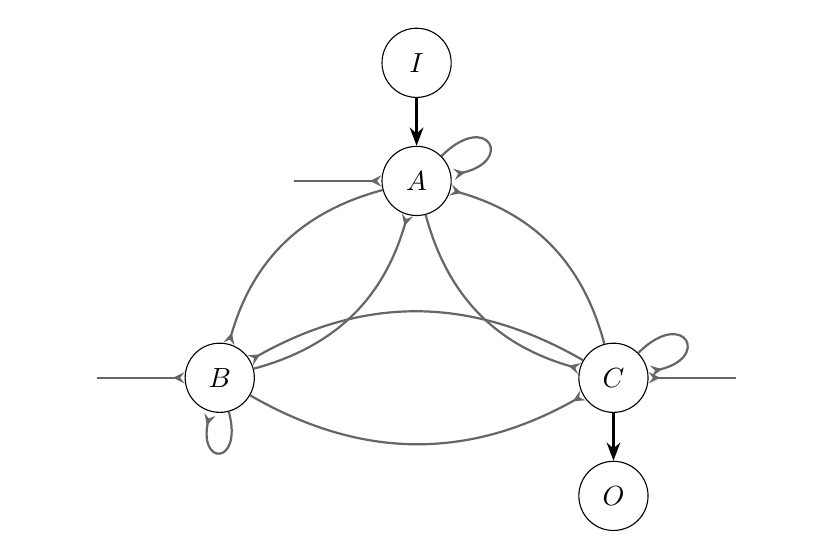
\begin{tikzpicture}

\node (EA) [state, style={draw=none}] at (0.5,2.5) {};
\node (EB) [state, style={draw=none}] at (-2,0) {};
\node (EC) [state, style={draw=none}] at (7,0) {};
\node (A) [state] at (2.5,2.5) {$A$};
\node (B) [state] at (0,0) {$B$};
\node (C) [state] at (5,0) {$C$};
\node (I) [state] at (2.5,4.0) {$I$};
\node (O) [state] at (5,-1.5) {$O$};

%Unknown:
\path [thick,every loop/.append style=-{Latex[length=2mm]},every loop/.append style=-{stealth reversed}]
(A) edge [in =10, out=45, loop,color=gray!80!black] (A)
(B) edge [loop below,color=gray!80!black] ()
(C) edge [in =10, out=45, loop,color=gray!80!black] (C)
(A) edge [bend right, -stealth reversed,color=gray!80!black] (C)
(A) edge [bend right, -stealth reversed,color=gray!80!black] (B)
(B) edge [bend right, -stealth reversed,color=gray!80!black] (A)
(B) edge [bend right, -stealth reversed,color=gray!80!black] (C)
(C) edge [bend right, -stealth reversed,color=gray!80!black] (A)
(C) edge [bend right, -stealth reversed,color=gray!80!black] (B)
(EB) edge [-stealth reversed, color=gray!80!black] (B)
(EA) edge [-stealth reversed, color=gray!80!black] (A)
(EC) edge [-stealth reversed, color=gray!80!black] (C)
(I) edge [-Stealth, color=black] (A)
(C) edge [-Stealth, color=black] (O)
;

\end{tikzpicture}
\end{document}